\RequirePackage{plautopatch}
\documentclass[uplatex,dvipdfmx,a4paper,10pt]{jsarticle}
\usepackage{graphicx}
\usepackage{amsmath}
\usepackage{mathcomp}
\usepackage{csvsimple}
\usepackage{siunitx}
\usepackage{url}


\title{重力加速度の測定}
\author{電気通信大学 I\hspace{-1.2pt}I\hspace{-1.2pt}I類\\
2313213 山口海音}
\date{\today}

\begin{document}

\maketitle

\section{目的}
地表において，自由落下するときの加速度で空気抵抗の影響を除いたものを大きさにもち，糸の先に鉛をつけて糸がさすものと同じ方向の加速度を重力加速度という．今回は重力加速度の大きさを，モデルによる計算値と実験値，文献値を比較する．この重力加速度の大きさにおいては万有引力の影響が支配的であるが，地球の自転による遠心力の影響が現れる精度で測定するために合致法を用いる．

\section{原理}

\subsection{重力加速度の推定}

    地球と地表の物体は互いに万有引力で引き合っている．さらに地表の物体は，地球の自転による遠心力を受けている．図\ref{fig:earth}のように，この$2$つの力の和を重力と見做すとき，重力加速度は以下のように表せる．

\begin{align}
    g 
    &= \left( \left( G\frac{M}{R^2}  - R\omega^2\cos^2{\phi} \right)^2 + \left( R\omega^2\sin^2{\phi} \right) \right)^{1/2}\\
    &= G\frac{M}{R^2} \left( 1 - 2\frac{ R\omega^2\cos^2\phi }{ G\dfrac{M}{R^2} } + \left( \frac{ R\omega^2\cos\phi }{ G\dfrac{M}{R^2} } \right)^2 \right)^{1/2}\\
    &\approx G\frac{M}{R^2} \left( 1 - \frac{ R\omega^2\cos^2\phi }{ G\dfrac{M}{R^2} } \right)\\
    &= G\frac{M}{R^2} - R\omega^2\cos^2\phi
\end{align}

\begin{figure}[htbp]
    \begin{center}
        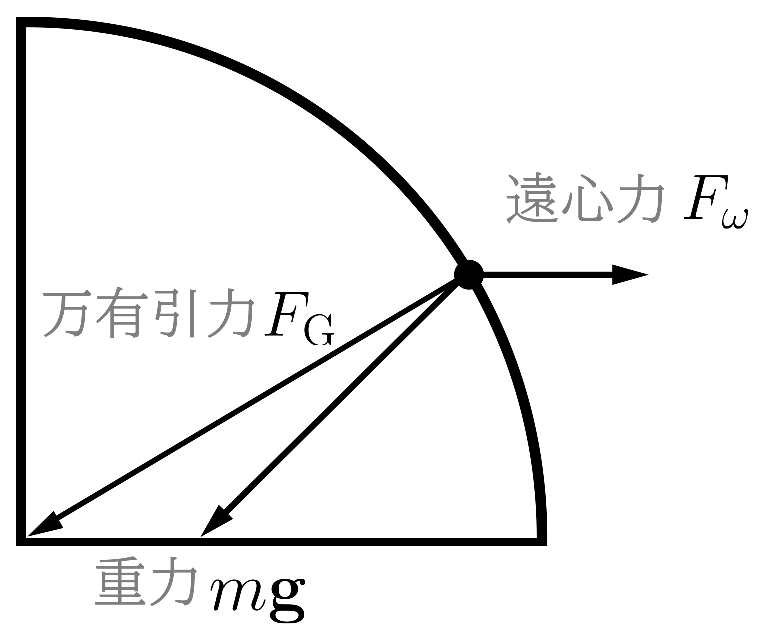
\includegraphics[width=5cm]{material/figure.eps}
        \caption{万有引力と遠心力による重力}
        \label{fig:earth}
    \end{center}
\end{figure}

\subsection{重力加速度の測定}

重力加速度は，様々な方法で測定されてきた（\cite{jihou}）．今回は振り子を用いた測定を行う．一端を固定し，もう一端におもりを付けた振り子の運動は，固定した点を中心，鉛直方向に始線をとった極座標で考えると以下のように表せる．

\begin{equation}
    mh\ddot{\theta} = -mg\sin{\theta} - \lambda h\dot{\theta}
\end{equation}

よって以下のような$\theta$についての$2$階微分方程式が解ければよい．

\begin{equation}\label{eq:basic}
    0 = \ddot{\theta} + \frac{\lambda}{m}\dot{\theta} + \frac{g}{h}\sin{\theta}
\end{equation}

ここで空気抵抗を無視し，$\sin{\theta} \approx \theta$とし，$\omega = \sqrt{\frac{g}{h}}$とすると，以下のように解ける．

\begin{equation}
    \theta = A\sin\left( \omega t + \alpha \right)
\end{equation}

よって，振り子の運動の周期は以下のようにあらわされる．

\begin{equation}
    T = 2\pi\sqrt{\frac{g}{h}}
\end{equation}

\subsubsection{精密測定}

式(\ref{eq:basic})をより良い近似で解くと，振り子の運動の周期は次のように表される．

\begin{equation}
    T = 2\pi\sqrt{\frac{h}{g}\left( 1 + \frac{2r^2}{5h^2} \right)}
\end{equation}

よって重力加速度$g$は，周期$T$がわかれば以下のように求められる．

\begin{equation}
    g = \frac{4\pi^2h}{T^2}\left( 1 + \frac{2r^2}{5h^2} + \frac{\theta^2}{8} \right)
\end{equation}

\section{実験方法}

第$1$に，実験装置のナイフエッヂの固定面から，振幅を図るための定規の上側までの距離lを測る．第$2$に金属球の直径をノギスで測る．第$3$に，約$1\si{\meter}$の糸を用意．一端に金属球を取り付け，もう一端を装置に取り付け，ナイフエッヂの固定面から金属球の最下部までの距離$h'$を測る．第$4$に，LEDフラッシュを$6$桁の精度で$2s$毎に発光させる．これが吊り糸を照らし，その位置が変化するときの周期$\tau$を観測する．

\section{実験結果}

先ず，今回の実験に用いた金属球の直径$d$を何度か測った結果をを表\ref{tb:metal-sph}に示す．

\begin{table}[htbp]
    \begin{center}
        \caption{金属球の直径}
        \label{tb:metal-sph}
        \begin{tabular}{r}
            \hline
            金属球の直径$d_i/\si{\meter}$\\
            \hline
            \csvreader[late after line=\\]{material/data-d.csv}
            {d=\d}
            {\d}
            \hline
        \end{tabular}
    \end{center}
\end{table}

次に，今回の実験で用いた振り子の，支点から金属球の最下部までの距離$h'$を何度か測った結果を表\ref{tb:h}に示す．

\begin{table}[htbp]
    \begin{center}
        \caption{振り子の，支点から金属球の最下部までの距離}
        \label{tb:h}
        \begin{tabular}{r}
            \hline
            距離$h'_i/\si{\meter}$\\
            \hline
            \csvreader[late after line=\\]{material/data-raw1h.csv}
            {h'=\h}
            {\h}
            \hline
        \end{tabular}
    \end{center}
\end{table}

次に，得られた周期$\tau_i$を\ref{tb:tau}に示す．

\begin{table}[htbp]
    \begin{center}
        \caption{周期}
        \label{tb:tau}
        \begin{tabular}{r}
            \hline
            周期$\tau_i/\si{\second}$\\
            \hline
            \csvreader[late after line=\\]{material/data-raw1tau.csv}
            {tau=\tau}
            {\tau}
            \hline
        \end{tabular}
    \end{center}
\end{table}

次に，得られた振れ幅$a_i$を\ref{tb:a}に示す．\newpage

\begin{table}[htbp]
    \begin{center}
        \caption{振れ幅}
        \label{tb:a}
        \begin{tabular}{r}
            \hline
            振れ幅$a_i/\si{\meter}$\\
            \hline
            \csvreader[late after line=\\]{material/data-raw1a.csv}
            {a=\a}
            {\a}
            \hline
        \end{tabular}
    \end{center}
\end{table}

ここまでの実験結果から得られるそれぞれのデータの平均値と不確かさ，今回の実験に用いた器具のデータ，即ち，振り子の支点から振れ幅を図る定規までの距離$l$と，LEDフラッシュの時間間隔$T_0$を表\ref{tb:data1_1}に示す．

\begin{table}[htbp]
    \begin{center}
        \caption{得られたデータ}
        \label{tb:data1_1}
        \begin{tabular}{r|rr}
            \hline
            データ名$X$ & 平均値$\langle X \rangle$ & 不確かさ$\Delta X$\\
            \hline
            \csvreader[late after line=\\]{material/data-data1_1.csv}
            {data=\data,mean=\mean,uc=\uc}
            {$\data$ & $\mean$ & $\uc$}
            \hline
        \end{tabular}
    \end{center}
\end{table}

ここまででえられたデータから振り子の振れ角$\theta$，金属球の半径$r$，振り子の，支点から質点近似したときの質点までの距離$h$，振り子の周期$T$を計算すると表\ref{tb:data1_2}のようになった．

\begin{table}[htbp]
    \begin{center}
        \caption{得られたデータからの計算値}
        \label{tb:data1_2}
        \begin{tabular}{r|rr}
            \hline
            データ名$X$ & 平均値$\langle X \rangle$ & 不確かさ$\Delta X$\\
            \hline
            \csvreader[late after line=\\]{material/data-data1_2.csv}
            {data=\data,mean=\mean,uc=\uc}
            {$\data$ & $\mean$ & $\uc$}
            \hline
        \end{tabular}
    \end{center}
\end{table}

ここまでの結果から重力加速度は次のように求められた．

\begin{align}
    g = 9.797\si{\meter\second^{-2}} && \Delta g = 0.01\si{\meter\second^{-2}}
\end{align}

\section{調査結果}

日本各地の緯度と重力実測値を表\ref{tb:geoinf}に示す（\cite{sci}）．ただし，$ \mathrm{mGal} = 10^{-5} \mathrm{ms^{-2}} $である．

\begin{table}[htbp]
    \begin{center}
        \caption{日本各地の地理情報}
        \label{tb:geoinf}
        \begin{tabular}{r|rrr}
            \hline
            地名 & 緯度[° ' ''] & 経度[° ' ''] & 重力実測値[$\mathrm{mGal}$]\\
            \hline
            \csvreader[late after line=\\]{material/search.csv}
            {name=\name,ido=\ido,kei=\kei,gra=\gra}
            {\name & \ido & \kei & \gra}
            \hline
        \end{tabular}
    \end{center}
\end{table}

\section{考察}

実験結果の重力加速度は，調査結果の羽田に非常に近い値となったが，不確かさが3桁になってしまった．文献値に対する実験値の誤差率は以下に示すとおりである．

\begin{align}
    \epsilon &= \dfrac{9.797-979759.54}{979759.54}\\
    &= -6.077 \times 10^{-5}\\
    \Delta \epsilon &= \frac{\Delta g}{979759.54}\\
    &=1\times 10 ^{-3}
\end{align}

\begin{thebibliography}{99}
    \bibitem{phy} \verb|伊東敏雄，『な～るほど！の力学』，東京学術図書出版社2003．|
    \bibitem{jihou} \verb|国土地理院，『国土地理院時報』，131集，国土地理院，2018．|
    \bibitem{sci} \verb|『日本各地の重力実測値』，理科年表プレミアム - コンテンツ表示，理科年表オフィシャルサイト(国立天文台・丸善出版)，2023-07-13閲覧．|
    \bibitem{keido} \verb|『東京都 市区町村の役所・役場及び東西南北端点の経度緯度(世界測地系)』，国土地理院，2023-07-14閲覧，https://www.gsi.go.jp/common/000230949.pdf．|
\end{thebibliography}


\end{document}